\chapter{Constructors, \texttt{self} Keyword, and Instance Variables}

\section{Introduction: Real-Life Hook}

Rahim created a \texttt{Student} class in the previous chapter.
Every time he created a student object, he had to manually set the name and marks.

He wondered:
``Can the object set its own data when it is created?  
Why does every method use the word \texttt{self}?''

To answer these questions, we need to understand:
\begin{itemize}
    \item Constructors
    \item The \texttt{self} keyword
    \item Instance variables
\end{itemize}

These ideas are the \textbf{foundation of Object-Oriented Programming}.

\section{Concept: What Is a Constructor?}

\begin{definition}{Constructor}
A constructor is a \textbf{special method that runs automatically when an object is created}.
\end{definition}

In Python, the constructor is named:

\begin{center}
\texttt{\_\_init\_\_}
\end{center}

Example:
\begin{verbatim}
class Student:
    def __init__(self):
        print("Student object created")
\end{verbatim}

\begin{verbatim}
s1 = Student()
\end{verbatim}

The message is printed automatically when the object is created.

\section{Why Do We Use Constructors?}

\begin{itemize}
    \item To initialize data
    \item To avoid writing extra code
    \item To ensure objects start in a valid state
\end{itemize}

Constructors make programs:
\begin{itemize}
    \item Cleaner
    \item Safer
    \item More professional
\end{itemize}

\section{Concept: What Is the \texttt{self} Keyword?}

\begin{definition}{\texttt{self}}
\texttt{self} refers to the \textbf{current object} inside a class.
\end{definition}

Think of \texttt{self} as saying:
\begin{center}
``This object’s own data''
\end{center}

Example:
\begin{verbatim}
class Student:
    def display(self):
        print("This is a student")
\end{verbatim}

Here, \texttt{self} tells Python which object is calling the method.

\section{Why Is \texttt{self} Important?}

\begin{itemize}
    \item It distinguishes object data from local variables
    \item It allows each object to have its own values
    \item Without \texttt{self}, Python cannot access instance variables
\end{itemize}

\section{Concept: Instance Variables}

\begin{definition}{Instance Variables}
Instance variables are \textbf{variables that belong to an object}, not the class.
\end{definition}

They are created using \texttt{self}.

Example:
\begin{verbatim}
class Student:
    def __init__(self, name, marks):
        self.name = name
        self.marks = marks
\end{verbatim}

Each object has its \textbf{own copy} of these variables.

\section{Creating Objects with Instance Variables}

\begin{verbatim}
s1 = Student("Ayesha", 80)
s2 = Student("Rafi", 45)

print(s1.name)
print(s2.name)
\end{verbatim}

Even though both objects use the same class:
\begin{itemize}
    \item Their data is different
    \item Their instance variables are separate
\end{itemize}

\section{Using Instance Variables Inside Methods}

\begin{verbatim}
class Student:
    def __init__(self, name, marks):
        self.name = name
        self.marks = marks

    def result(self):
        if self.marks >= 40:
            print(self.name, "has passed")
        else:
            print(self.name, "has failed")
\end{verbatim}

\section{Mini-Project: Student Profile Creator}

\textbf{Goal:} Automatically create and display student profiles.

\begin{verbatim}
class Student:
    def __init__(self, name, roll, marks):
        self.name = name
        self.roll = roll
        self.marks = marks

    def display(self):
        print("Name:", self.name)
        print("Roll:", self.roll)
        print("Marks:", self.marks)

s1 = Student("Ayesha", 5, 88)
s2 = Student("Rahim", 8, 67)

s1.display()
s2.display()
\end{verbatim}

Students learn:
\begin{itemize}
    \item How constructors initialize data
    \item How \texttt{self} connects data to objects
    \item How instance variables store object information
\end{itemize}

\section{Diagram: Object Creation with Constructor}

\begin{center}
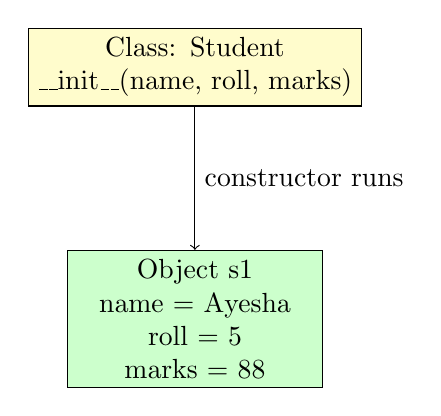
\begin{tikzpicture}[node distance=1.7cm]
\node (class) [draw, rectangle, fill=yellow!20, text width=4cm, align=center] {Class: Student\\
\_\_init\_\_(name, roll, marks)};
\node (obj) [draw, rectangle, fill=green!20, below of=class, yshift=-1.5cm, text width=3cm, align=center] {Object s1\\
name = Ayesha\\
roll = 5\\
marks = 88};

\draw[->] (class) -- node[right]{constructor runs} (obj);
\end{tikzpicture}
\end{center}

\section{Common Beginner Mistakes}

\begin{itemize}
    \item Forgetting to use \texttt{self}
    \item Using local variables instead of instance variables
    \item Passing wrong number of arguments to constructor
\end{itemize}

\section{Key Concepts}

\begin{itemize}
    \item Constructor initializes objects
    \item \texttt{\_\_init\_\_} runs automatically
    \item \texttt{self} refers to the current object
    \item Instance variables store object-specific data
\end{itemize}

\section{End-of-Chapter Exercises}

\subsection{Very Short Questions}

\begin{enumerate}
    \item What is a constructor?
    \item Which method is used as a constructor in Python?
    \item What does \texttt{self} refer to?
\end{enumerate}

\subsection{Short Answer Questions}

\begin{enumerate}
    \item Explain why \texttt{self} is necessary.
    \item Differentiate between local variables and instance variables.
    \item Write a class with a constructor that stores two numbers.
\end{enumerate}

\subsection{Activity-Based Exercises}

\begin{enumerate}
    \item Create a \texttt{Book} class with title and price using a constructor.
    \item Design a \texttt{BankAccount} class with account holder name and balance.
    \item Modify the Student class to calculate grade using marks.
\end{enumerate}

\section{Teacher Notes}

\marginnote{
\textbf{Learning Objectives}
\begin{itemize}
    \item Students understand constructors and initialization
    \item Students correctly use \texttt{self}
    \item Students work with instance variables
\end{itemize}

\textbf{Teaching Tips}
\begin{itemize}
    \item Use real-life analogies (birth form = constructor)
    \item Emphasize ``each object has its own data''
    \item Debug common mistakes together
\end{itemize}

\textbf{Assessment}
\begin{itemize}
    \item Proper constructor usage
    \item Correct access to instance variables
\end{itemize}
}